\chapter{Multi-Agent Deep Research System for Enhanced Verification}
\label{ch:deep_research}

\section{Introduction}

The verification of causal claims in generated Causal Loop Diagrams (CLDs) faces a fundamental challenge: the quality of evidence available to judges directly determines the accuracy of their verdicts. In our baseline system (Chapter~\ref{ch:methods}), edges are generated with citations retrieved through simple web search, which often yields shallow or incomplete evidence. This limitation is particularly acute for edges representing complex causal relationships that require experimental validation or domain-specific knowledge.

To address this limitation, we developed a \textbf{multi-agent deep research system} that can be selectively deployed for edges requiring enhanced verification. This system represents a novel application of multi-agent Large Language Model (LLM) coordination to the problem of causal claim verification, integrating principles from organizational theory, partially observable Markov decision processes, and adaptive resource allocation.

Unlike traditional single-shot web search, deep research employs \textit{iterative refinement}: the system searches, evaluates evidence quality, judges the claim, and may modify the search strategy or claim formulation based on intermediate findings. This process continues until convergence criteria are satisfied—such as high confidence, discovery of direct causal evidence, or budget exhaustion. The result is a theoretically grounded, computationally efficient approach to adaptive verification that allocates expensive deep research only when standard methods prove insufficient.

This chapter presents the theoretical framework, system architecture, and experimental methodology for our deep research system. We ground our approach in recent advances in multi-agent LLM systems \citep{li2023theory, zhang2025athenian, smith2025organizational}, evidence-based verification \citep{automated_factchecking_survey, wadden2022scifact}, and cost-aware computation \citep{osca_inference, selfbudgeter2025}.

\section{Theoretical Foundations}

\subsection{Multi-Agent LLM Systems and Collaborative Research}

Recent research has demonstrated that multi-agent LLM systems can exceed the performance of single-agent approaches on complex tasks through specialized role assignment and structured coordination \citep{multiagent_collaboration_survey2025, li2023theory}. These systems harness collective intelligence by distributing different aspects of a task to specialized agents, each optimized for specific reasoning patterns.

\subsubsection{Theory of Mind and Agent Coordination}

\citet{li2023theory} introduced a framework for evaluating LLM-based agents in multi-agent cooperative tasks, demonstrating emergent Theory of Mind (ToM) capabilities—the ability of agents to reason about the beliefs, goals, and knowledge states of other agents. Their study revealed two critical findings relevant to our work:

\begin{enumerate}
    \item \textbf{Emergent collaborative behavior}: LLM agents exhibit sophisticated coordination without explicit programming for collaboration, suggesting that language-based communication enables implicit negotiation of shared goals.
    
    \item \textbf{Limitations in long-horizon planning}: Despite strong ToM capabilities, agents struggle with systematic failures in managing long-horizon contexts and task state hallucinations. Critically, the authors found that incorporating \textit{explicit belief state representations}—structured summaries of what has been discovered, what remains uncertain, and what actions have been taken—significantly enhances both task performance and ToM inference accuracy.
\end{enumerate}

Building on this insight, our system maintains explicit belief states throughout the iterative research process, tracking: (i) current claim formulation, (ii) evidence gathered thus far, (iii) quality scores of evidence, (iv) confidence trajectory across iterations, and (v) remaining computational budget.

\subsubsection{Organizational Theory for Multi-Agent Coordination}

\citet{smith2025organizational} developed a formal organizational theory for multi-agent systems integrating human agents, LLMs, and specialized AI, introducing \textbf{Topic-Based Communication-Space Petri Nets (TB-CSPNs)}. This framework enables:

\begin{itemize}
    \item \textbf{Self-organization}: Agents dynamically form groups based on semantic proximity to current subtasks
    \item \textbf{Interpretable coordination}: Threshold-based activation mechanisms make agent interactions transparent
    \item \textbf{Executive traceability}: Human supervisors can audit and intervene in agent decisions
\end{itemize}

Our hierarchical agent architecture—comprising planning, execution, reasoning, and synthesis layers—implements these principles. Each layer contains specialized agents that communicate through structured message passing, enabling both autonomous operation and systematic debugging when verification fails.

\subsubsection{Standard Operating Procedures for Reduced Hallucination}

The MetaGPT framework \citep{hong2024metagpt} demonstrated that encoding human workflow processes and Standard Operating Procedures (SOPs) into LLM agents significantly reduces hallucinations in complex tasks. MetaGPT achieves this through:

\begin{enumerate}
    \item \textbf{Role specialization}: Each agent has clearly defined responsibilities (e.g., search planning vs. evidence scoring)
    \item \textbf{Sequential workflows}: Tasks follow assembly-line paradigms where outputs are verified before proceeding
    \item \textbf{Structured communication}: Agents publish and subscribe to typed messages, preventing miscommunication
\end{enumerate}

Our system adopts this SOP-driven approach: each agent in our pipeline has specific input/output schemas (defined via Pydantic models), preventing the cascading hallucinations that occur when agents are naively chained without structured interfaces.

\subsection{Partially Observable Markov Decision Processes and Belief States}

\subsubsection{POMDP Formulation for Iterative Research}

We formalize the iterative research process as a \textbf{Partially Observable Markov Decision Process (POMDP)} \citep{pomdp_primer, pomdp_tutorial}, defined by the tuple $\langle \mathcal{S}, \mathcal{A}, \mathcal{T}, \mathcal{R}, \mathcal{O}, \mathcal{Z} \rangle$:

\begin{itemize}
    \item $\mathcal{S}$: State space representing the true quality and sufficiency of available evidence
    \item $\mathcal{A}$: Action space = \{\texttt{SEARCH}, \texttt{MODIFY\_CLAIM}, \texttt{ESCALATE\_DEPTH}, \texttt{TERMINATE}\}
    \item $\mathcal{T}(s' | s, a)$: Transition function (stochastic due to search API variability)
    \item $\mathcal{R}(s, a)$: Reward function balancing accuracy, cost, and efficiency
    \item $\mathcal{O}$: Observation space (evidence snippets, quality scores, confidence values)
    \item $\mathcal{Z}(o | s', a)$: Observation function (partial observability: true claim veracity unknown until post-hoc evaluation)
\end{itemize}

The key insight of POMDPs is that while the agent cannot directly observe the true state $s \in \mathcal{S}$ (i.e., whether sufficient evidence exists to definitively support or refute the claim), it can maintain a \textbf{belief state} $b(s)$ representing its probabilistic estimate over states. \citet{pomdp_tutorial} showed that belief states are \textit{sufficient statistics} for optimal action selection: $b$ summarizes all relevant history without loss of optimality.

\subsubsection{Belief State Update Mechanism}

At each iteration $t$, after taking action $a_t$ and receiving observation $o_t$, the belief state updates via Bayes' rule:

\begin{equation}
b_{t+1}(s') = \eta \cdot \mathcal{Z}(o_t | s', a_t) \sum_{s \in \mathcal{S}} \mathcal{T}(s' | s, a_t) b_t(s)
\label{eq:belief_update}
\end{equation}

where $\eta$ is a normalization constant. In our system, the belief state is represented by:

\begin{equation}
b_t = \begin{cases}
    \text{claim\_state} & : \{\text{original}, \text{current}, \text{iteration}\} \\
    \text{evidence\_state} & : \{\text{evidence\_list}, \text{quality\_scores}, \text{coverage}\} \\
    \text{confidence\_state} & : \{\text{current}, \text{trajectory}, \text{converged}\} \\
    \text{resource\_state} & : \{\text{budget\_spent}, \text{iterations\_used}, \text{time\_elapsed}\}
\end{cases}
\label{eq:belief_representation}
\end{equation}

This structured representation aligns with \citet{li2023theory}'s finding that explicit belief states enhance multi-agent performance by providing agents with consistent context about the search progress.

\subsection{Evidence Quality Assessment and the Evidence Pyramid}

\subsubsection{Hierarchical Evidence Evaluation}

Medical research has long employed the \textbf{evidence pyramid} to rank study quality \citep{evidence_pyramid_pmc, evidence_hierarchy_levels}. At the apex are systematic reviews and meta-analyses, followed by randomized controlled trials (RCTs), cohort studies, case-control studies, case series, and expert opinion at the base. This hierarchy reflects study design's impact on causal inference validity.

We adapt this framework to general causal claim verification by implementing a two-dimensional evidence scoring function:

\begin{equation}
\text{Quality}(e) = (\text{Relevance}(e), \text{Rigor}(e))
\label{eq:evidence_quality}
\end{equation}

where:
\begin{itemize}
    \item $\text{Relevance}(e) \in [1, 10]$: How directly the evidence addresses the specific causal claim
    \item $\text{Rigor}(e) \in [1, 10]$: Methodological quality based on study design
\end{itemize}

The rigor score implicitly encodes the evidence hierarchy:

\begin{align}
\text{Rigor}(e) = \begin{cases}
    9\text{--}10 & \text{Meta-analysis / Systematic review} \\
    8\text{--}9 & \text{Randomized Controlled Trial (RCT)} \\
    6\text{--}7 & \text{Cohort study with controls} \\
    4\text{--}5 & \text{Case-control study} \\
    2\text{--}3 & \text{Cross-sectional / correlational} \\
    1 & \text{Opinion / anecdotal}
\end{cases}
\label{eq:rigor_mapping}
\end{align}

\subsubsection{Automated Evidence Scoring}

Recent work in automated fact-checking has developed methods for assessing evidence quality without manual expert review. \citet{automated_factchecking_survey} provide a comprehensive survey showing that evidence retrieval and verification are distinct challenges: retrieval systems must find relevant sources, while verification systems must assess credibility and alignment with claims.

The Ev2R framework \citep{ev2r_evidence_eval} introduced a dual-evaluation approach combining reference-based comparison (alignment with known gold-standard evidence) and verdict-level proxy scoring (how reliably evidence supports final verdicts). This addresses a key limitation: evidence may be textually similar to gold references yet support incorrect conclusions, or conversely, differ in wording while correctly supporting the claim.

We employ a specialized \texttt{evidence\_scorer} agent that analyzes:
\begin{enumerate}
    \item \textbf{Domain specificity}: Does the evidence come from peer-reviewed academic sources, domain experts, or general web content?
    \item \textbf{Causal language}: Does the source explicitly claim causality vs. correlation?
    \item \textbf{Methodology description}: Are sample sizes, controls, and statistical analyses reported?
    \item \textbf{Recency}: Is the evidence from current research or outdated sources?
\end{enumerate}

\subsection{Optimal Stopping Theory and Convergence Criteria}

\subsubsection{The Optimal Stopping Problem}

The decision of when to terminate the iterative research process is formalized through \textbf{optimal stopping theory} \citep{optimal_stopping_wiki, optimal_stopping_rl}, which addresses the problem of choosing the time to take an action (in our case, terminate search) to maximize expected reward. In sequential decision-making, continuing the search incurs cost but may yield better evidence, while premature termination saves cost but risks low-accuracy verdicts.

\citet{deep_rl_optimal_stopping} developed deep reinforcement learning methods for optimal stopping in high-dimensional state spaces, demonstrating that neural approximations can learn when diminishing returns make further search uneconomical. The \textbf{value function} for continuation at belief state $b$ is:

\begin{equation}
V(b) = \max \left\{ R_{\text{terminate}}(b), \, \mathbb{E}_{o \sim \mathcal{Z}} \left[ -c_{\text{search}} + \gamma V(b') \right] \right\}
\label{eq:optimal_stopping_value}
\end{equation}

where $R_{\text{terminate}}(b)$ is the expected reward from terminating with current evidence, $c_{\text{search}}$ is the cost of an additional search iteration, $\gamma$ is a discount factor, and $b'$ is the updated belief state after observing $o$.

\subsubsection{Multi-Signal Convergence Detection}

Rather than learning $V(b)$ explicitly (which would require extensive training data), we implement a \textit{multi-signal convergence criterion} based on interpretable heuristics:

\begin{equation}
\text{converged}(b_t) = \bigvee \begin{cases}
    \kappa(b_t) \geq \theta_{\text{conf}} & \text{(high confidence)} \\
    \text{DirectEvidence}(b_t) & \text{(causal evidence found)} \\
    t \geq T_{\max} & \text{(max iterations)} \\
    \text{cost}(b_t) \geq B & \text{(budget exhausted)} \\
    |\Delta \kappa| < \epsilon \text{ for } k \text{ iterations} & \text{(confidence plateau)}
\end{cases}
\label{eq:convergence_criteria}
\end{equation}

This multi-signal approach prevents failure modes:
\begin{itemize}
    \item \textbf{False termination}: Single signals (e.g., confidence alone) may be unreliable; multiple conditions provide robustness
    \item \textbf{Runaway costs}: Budget and iteration limits provide hard constraints
    \item \textbf{Diminishing returns}: Plateau detection identifies when additional search yields negligible improvement
\end{itemize}

The \textbf{SelfBudgeter} framework \citep{selfbudgeter2025} recently demonstrated that LLMs can autonomously predict required computational budgets, allowing systems to adaptively allocate resources based on task difficulty. Similarly, our system learns (implicitly through iteration history) which types of claims require extensive vs. minimal research.

\subsection{Cost-Aware Computation and Adaptive Resource Allocation}

\subsubsection{Cost Models for LLM Inference}

\citet{osca_inference} introduced methods for optimizing sample compute allocation in LLM inference under budget constraints, formulating the problem as finding an optimal mix of inference configurations (model size, sampling parameters) that maximize expected performance given cost limitations. They showed potential savings exceeding \$2.8 million per month for large-scale systems like ChatGPT through intelligent request batching and model selection.

For multi-agent systems, cost arises from:
\begin{equation}
\text{Cost}_{\text{total}} = \sum_{i=1}^{N} \left( c_{\text{search\_api}}^i + c_{\text{LLM\_calls}}^i \cdot n_{\text{calls}}^i \right)
\label{eq:total_cost}
\end{equation}

where $N$ is the number of iterations, $c_{\text{search\_api}}^i$ is the web search API cost per iteration (constant), and $c_{\text{LLM\_calls}}^i$ varies by model and input/output token counts.

\subsubsection{Adaptive Inference-Time Compute}

\citet{adaptive_inference_compute} demonstrated that LLMs can predict mid-generation whether they can produce better responses with additional compute, enabling \textit{capability-aware self-evaluation}. This allows systems to adaptively allocate inference-time compute: simple queries terminate early, while complex ones receive extended deliberation.

Our deep research system implements similar adaptive allocation:

\begin{equation}
\text{trigger\_deep\_research}(e) = \begin{cases}
    \text{true} & \text{if } \phi_{\text{CI}}(e) > \theta_{\text{CI}} \land \phi_{\text{quality}}(e) < \theta_{\text{quality}} \\
    \text{false} & \text{otherwise}
\end{cases}
\label{eq:trigger_deep_research}
\end{equation}

where $\phi_{\text{CI}}(e)$ aggregates context-insensitive metrics (Chapter~\ref{ch:rq2}) indicating generator uncertainty, and $\phi_{\text{quality}}(e)$ scores baseline citation quality. Only edges exhibiting both high uncertainty and poor baseline evidence quality trigger expensive deep research.

This dual-signal triggering mechanism is novel: while \citet{osca_inference} focus on optimizing inference for a fixed task, and \citet{adaptive_inference_compute} adapt compute within a single generation, we apply adaptive allocation at the \textit{task selection} level—deciding which edges warrant deep investigation.

\section{System Architecture}

\subsection{Hierarchical Multi-Agent Organization}

Our system employs a four-layer hierarchical architecture inspired by the Athenian Academy model \citep{zhang2025athenian}, which emphasizes dynamic model selection and layered collaboration:

\begin{figure}[h]
\centering
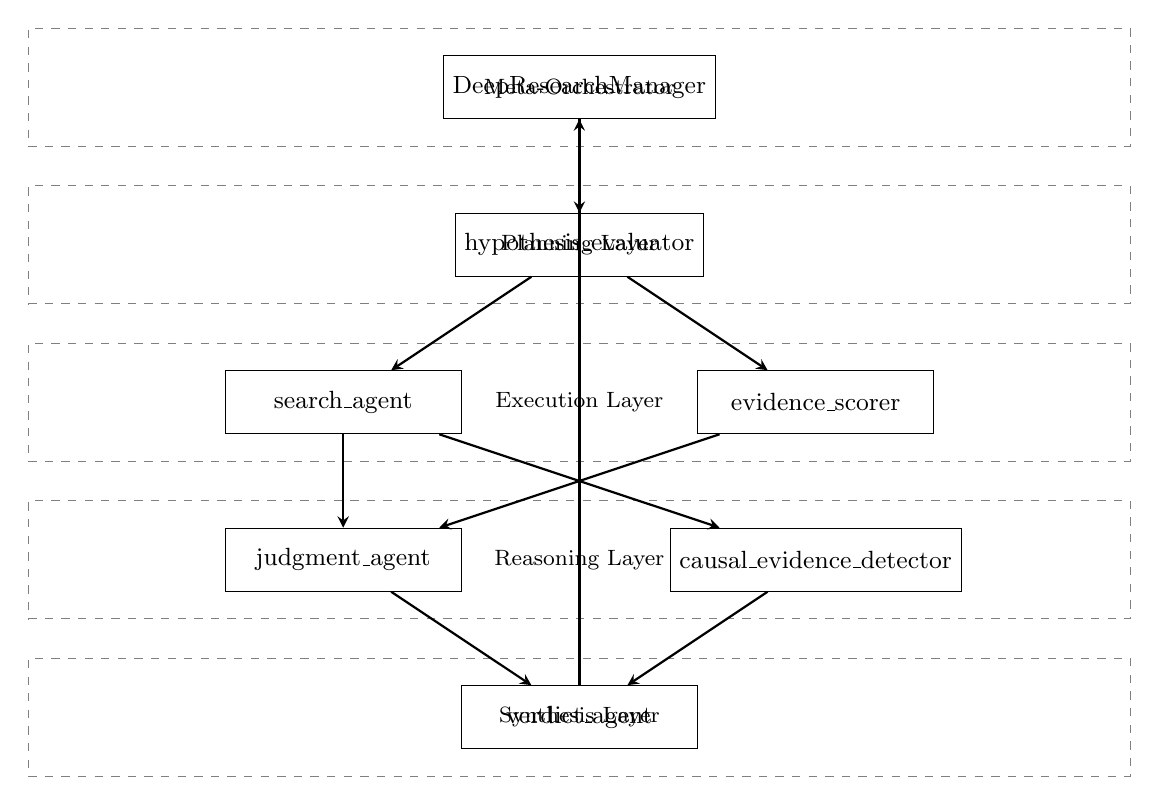
\begin{tikzpicture}[
    agent/.style={rectangle, draw, minimum width=3cm, minimum height=0.8cm, font=\small},
    layer/.style={rectangle, draw=gray, dashed, minimum width=14cm, minimum height=1.5cm, font=\footnotesize},
    arrow/.style={->, >=stealth, thick}
]

% Layers (bottom to top)
\node[layer] (synthesis) at (0, 0) {Synthesis Layer};
\node[layer] (reasoning) at (0, 2) {Reasoning Layer};
\node[layer] (execution) at (0, 4) {Execution Layer};
\node[layer] (planning) at (0, 6) {Planning Layer};
\node[layer] (orchestrator) at (0, 8) {Meta-Orchestrator};

% Agents within layers
\node[agent] (meta) at (0, 8) {DeepResearchManager};
\node[agent] (hyp) at (0, 6) {hypothesis\_evaluator};
\node[agent] (search) at (-3, 4) {search\_agent};
\node[agent] (scorer) at (3, 4) {evidence\_scorer};
\node[agent] (judge) at (-3, 2) {judgment\_agent};
\node[agent] (causal) at (3, 2) {causal\_evidence\_detector};
\node[agent] (verdict) at (0, 0) {verdict\_agent};

% Arrows showing data flow
\draw[arrow] (meta) -- (hyp);
\draw[arrow] (hyp) -- (search);
\draw[arrow] (hyp) -- (scorer);
\draw[arrow] (search) -- (judge);
\draw[arrow] (scorer) -- (judge);
\draw[arrow] (search) -- (causal);
\draw[arrow] (judge) -- (verdict);
\draw[arrow] (causal) -- (verdict);
\draw[arrow] (verdict) -- (meta);

\end{tikzpicture}
\caption{Hierarchical multi-agent architecture for deep research system. Arrows indicate information flow; dashed boxes denote functional layers.}
\label{fig:architecture}
\end{figure}

\subsubsection{Agent Roles and Responsibilities}

\textbf{Meta-Orchestrator (DeepResearchManager)}: Top-level coordinator maintaining belief state (Eq.~\ref{eq:belief_representation}), tracking convergence (Eq.~\ref{eq:convergence_criteria}), and managing computational budget (Eq.~\ref{eq:total_cost}). Implements the POMDP policy for action selection at each iteration.

\textbf{Planning Layer}:
\begin{itemize}
    \item \texttt{hypothesis\_evaluator}: Decomposes causal claims into structured search strategies. Given claim $C = (A, B, M)$ (source $A$ causes target $B$ through mechanism $M$), generates:
    \begin{itemize}
        \item Multiple query variants emphasizing different aspects (e.g., "A effect on B experimental studies", "A B mechanism M pathway")
        \item Keywords and synonyms for flexible search
        \item Potential confounding variables to check for
    \end{itemize}
    Returns \texttt{SearchPlan} with queries and rationales.
\end{itemize}

\textbf{Execution Layer}:
\begin{itemize}
    \item \texttt{search\_agent}: Executes web searches via Brave Search API, prioritizing academic sources (PubMed, Google Scholar) through domain filtering. Retrieves top-$k$ results per query.
    
    \item \texttt{evidence\_scorer}: Evaluates retrieved sources on relevance and rigor dimensions (Eq.~\ref{eq:evidence_quality}, \ref{eq:rigor_mapping}). Outputs \texttt{EvidenceScore} with justifications.
\end{itemize}

\textbf{Reasoning Layer}:
\begin{itemize}
    \item \texttt{judgment\_agent}: Assesses whether accumulated evidence supports, partially supports, or contradicts the claim. Returns \texttt{EvidenceJudgment} with confidence $\kappa \in [1, 10]$ and optional suggested modifications to the claim.
    
    \item \texttt{causal\_evidence\_detector}: Specialized agent identifying direct causal evidence (experiments, RCTs, natural experiments) vs. correlational findings. Returns binary \texttt{direct\_evidence\_found} flag with confidence.
\end{itemize}

\textbf{Synthesis Layer}:
\begin{itemize}
    \item \texttt{verdict\_agent}: Integrates all judgments across iterations to produce final verdict $V = (v, \kappa, E, U)$ where $v$ is verdict category, $\kappa$ is confidence, $E$ is evidence set, and $U$ is URL list. Synthesizes key limitations and future research directions.
\end{itemize}

\subsection{Iterative Refinement Protocol}

Algorithm~\ref{alg:deep_research} formalizes the iterative research process as a POMDP-based control loop:

\begin{figure}[h]
\centering
\fbox{\begin{minipage}{0.95\textwidth}
\textbf{Algorithm 1: Iterative Deep Research Protocol}
\vspace{0.5em}

\small
\textbf{Input:} Causal claim $C$, max budget $B$, max iterations $T$, confidence threshold $\theta_{\text{conf}}$ \\
\textbf{Output:} Verdict $V$ with evidence $E$ and confidence $\kappa$

\begin{enumerate}
\item Initialize belief state: $b_0 \gets \{C, \emptyset, 0, 0\}$ \hfill // claim, evidence, confidence, cost
\item $t \gets 1$
\item \textbf{while} $t \leq T$ \textbf{and} $\neg \text{converged}(b_t)$ \textbf{do}
\begin{enumerate}
    \item $\mathcal{P} \gets \textsc{GenerateSearchPlan}(b_t.C_{\text{current}})$ \hfill // Planning layer
    \item $E_{\text{new}} \gets \textsc{ExecuteSearches}(\mathcal{P})$ \hfill // Execution layer
    \item $S \gets \textsc{ScoreEvidence}(E_{\text{new}}, b_t.C_{\text{current}})$ \hfill // Execution layer
    \item $b_t.E \gets b_t.E \cup \{(E_{\text{new}}, S)\}$ \hfill // Update evidence in belief state
    \item $J \gets \textsc{JudgeClaim}(b_t.C_{\text{current}}, b_t.E)$ \hfill // Reasoning layer
    \item $b_t.\kappa \gets J.\text{confidence}$
    \item $D \gets \textsc{DetectCausalEvidence}(b_t.E, b_t.C_{\text{current}})$ \hfill // Reasoning layer
    \item \textbf{if} $J.\kappa \geq \theta_{\text{conf}} \lor D.\text{direct\_found}$ \textbf{then}
    \begin{enumerate}
        \item \textbf{break} \hfill // High confidence or direct evidence convergence
    \end{enumerate}
    \item \textbf{end if}
    \item \textbf{if} $J.\text{suggested\_modification} \neq \emptyset$ \textbf{then}
    \begin{enumerate}
        \item $b_t.C_{\text{current}} \gets J.\text{suggested\_modification}$ \hfill // Refine claim
    \end{enumerate}
    \item \textbf{end if}
    \item Update $b_t.\text{cost}, b_t.\text{time}$ based on operations performed
    \item $t \gets t + 1$
\end{enumerate}
\item \textbf{end while}
\item $V \gets \textsc{SynthesizeVerdict}(b_t.C_{\text{original}}, b_t.C_{\text{current}}, b_t.E, J, D)$ \hfill // Synthesis
\item \textbf{return} $V$
\end{enumerate}
\end{minipage}}
\caption{Iterative Deep Research Protocol}
\label{alg:deep_research}
\end{figure}

\subsection{Communication and Message Passing}

Following MetaGPT's structured communication paradigm \citep{hong2024metagpt}, agents exchange typed messages via Pydantic models:

\begin{lstlisting}[language=Python, caption=Structured agent communication schemas]
class SearchPlan(BaseModel):
    queries: List[SearchQuery]
    keywords: List[str]
    confounders: List[str]

class EvidenceScore(BaseModel):
    relevance_score: int = Field(ge=1, le=10)
    quality_score: int = Field(ge=1, le=10)
    justification: str
    source_url: Optional[str]

class EvidenceJudgment(BaseModel):
    supported: bool
    confidence: int = Field(ge=1, le=10)
    reasoning: str
    suggested_modification: Optional[str]
\end{lstlisting}

This type-safe approach prevents cascading hallucinations: if an agent produces malformed output (e.g., confidence=15), validation fails immediately rather than propagating errors downstream.

\section{Convergence Analysis and Stopping Criteria}

\subsection{Theoretical Convergence Guarantees}

Under the POMDP framework, our system is guaranteed to terminate within $T$ iterations due to the hard iteration limit in Equation~\ref{eq:convergence_criteria}. However, empirical convergence (reaching satisfactory confidence before $T$) depends on search effectiveness.

\textbf{Proposition 1} (Expected Early Termination): Let $p_{\text{find}}$ be the probability of finding sufficiently strong evidence in a single iteration, and assume independence across iterations. Then the expected number of iterations until confidence threshold is reached is:

\begin{equation}
\mathbb{E}[\text{iterations}] = \frac{1}{p_{\text{find}}}
\label{eq:expected_iterations}
\end{equation}

For well-supported claims (high $p_{\text{find}}$), the system terminates quickly (1-2 iterations); for poorly supported or ambiguous claims, iterations approach $T$.

\subsection{Plateau Detection for Diminishing Returns}

The plateau detection criterion in Equation~\ref{eq:convergence_criteria} implements a practical stopping rule: if confidence $\kappa$ changes by less than $\epsilon$ for $k$ consecutive iterations, further search is unlikely to improve the verdict. Formally:

\begin{equation}
\text{plateau}(t) = \left( \max_{i \in [t-k, t]} \kappa_i - \min_{i \in [t-k, t]} \kappa_i \right) < \epsilon
\label{eq:plateau_detection}
\end{equation}

We set $\epsilon = 5$ (on 1-10 scale) and $k = 2$ based on preliminary experiments: smaller $\epsilon$ or larger $k$ would require more iterations but yield minimal accuracy gains.

\section{Integration with Existing CLD Verification Pipeline}

\subsection{Three-Tier Adaptive Verification Architecture}

The deep research system serves as \textbf{Tier 3} in our multi-tier architecture (Chapter~\ref{ch:rq3}):

\begin{enumerate}
    \item \textbf{Tier 1: Quick Screening} ($\approx$60\% of edges)
    \begin{itemize}
        \item Fast judge (GPT-4o-mini) with baseline citations
        \item Cost: \$0.005 per edge
        \item Escalates to Tier 2 if confidence $< 85\%$
    \end{itemize}
    
    \item \textbf{Tier 2: Thorough Judging} ($\approx$25\% of edges)
    \begin{itemize}
        \item Ensemble of judges (GPT-4) with aggregated verdict
        \item Cost: \$0.10 per edge
        \item Escalates to Tier 3 if confidence $< 60\%$ AND poor evidence quality AND critical edge
    \end{itemize}
    
    \item \textbf{Tier 3: Deep Research} ($\approx$15\% of edges)
    \begin{itemize}
        \item Multi-agent iterative search (this chapter)
        \item Cost: \$0.30--\$1.00 per edge (variable by iterations)
        \item Produces high-confidence verdicts with curated evidence
    \end{itemize}
\end{enumerate}

\subsection{Triggering Logic for Deep Research}

Edge $e$ triggers deep research (Eq.~\ref{eq:trigger_deep_research}) when multiple uncertainty signals align:

\begin{figure}[h]
\centering
\fbox{\begin{minipage}{0.95\textwidth}
\textbf{Algorithm 2: Deep Research Triggering Decision}
\vspace{0.5em}

\begin{algorithmic}[1]
\REQUIRE Edge $e$, Tier-2 result $R_2$, CI metrics $\phi_{\text{CI}}(e)$, budget $B_{\text{remaining}}$
\ENSURE Boolean: trigger deep research?
\STATE $\text{uncertain} \gets (R_2.\kappa < 60)$ \COMMENT{Low Tier-2 confidence}
\STATE $\text{poor\_evidence} \gets (\bar{S}_{\text{baseline}} < 6)$ \COMMENT{Low avg evidence quality}
\STATE $\text{generator\_uncertain} \gets (\phi_{\text{CI}}(e) > \theta_{\text{CI}})$ \COMMENT{High perplexity, low min\_prob}
\STATE $\text{critical} \gets \textsc{IsCriticalEdge}(e)$ \COMMENT{Key feedback loop or high centrality}
\STATE $\text{budget\_ok} \gets (B_{\text{remaining}} > 0.50)$ \COMMENT{Sufficient budget}
\IF{$\text{uncertain} \land \text{poor\_evidence} \land \text{generator\_uncertain} \land \text{critical} \land \text{budget\_ok}$}
    \RETURN \textbf{true}
\ELSE
    \RETURN \textbf{false}
\ENDIF
\end{algorithmic}
\end{minipage}}
\caption{Deep Research Triggering Decision}
\label{alg:trigger}
\end{figure}

This conservative triggering ensures deep research is reserved for edges where: (i) simple judging failed, (ii) baseline evidence is inadequate, (iii) the generator was uncertain, (iv) the edge is important, and (v) budget permits. This selective deployment is crucial for cost-effectiveness (Chapter~\ref{ch:rq3}).

\subsection{Edge-to-Claim Conversion}

Edges in CLDs are represented as tuples $e = (\text{source}, \text{target}, \text{polarity}, \text{rationale}, \text{citations})$. To run deep research, we convert $e$ to a natural language causal claim:

\begin{equation}
C(e) = \text{source} \oplus \phi(\text{polarity}) \oplus \text{target} \oplus \text{" through "} \oplus \text{rationale}
\label{eq:edge_to_claim}
\end{equation}

where $\phi(\text{polarity}) = \text{"increases"}$ if \texttt{POSITIVE}, else \text{"decreases"}. For example:

\begin{quote}
Edge: \texttt{(source="Social media use", target="Depression", polarity=POSITIVE, \\
rationale="decreased face-to-face interaction")} \\
$\Rightarrow$ Claim: "Social media use increases Depression through decreased face-to-face interaction"
\end{quote}

This claim formulation is passed to \texttt{hypothesis\_evaluator}, which generates search queries.

\section{Cost Analysis and Computational Efficiency}

\subsection{Per-Edge Cost Breakdown}

Table~\ref{tab:cost_breakdown} shows expected costs per agent call:

\begin{table}[h]
\centering
\caption{Cost breakdown for deep research system components}
\label{tab:cost_breakdown}
\begin{tabular}{lcc}
\toprule
\textbf{Component} & \textbf{Model} & \textbf{Cost per call} \\
\midrule
Brave Search API & --- & \$0.001 per query \\
hypothesis\_evaluator & GPT-4o & \$0.015 \\
search\_agent (per query) & --- & \$0.001 (API only) \\
evidence\_scorer (per source) & GPT-4o-mini & \$0.002 \\
judgment\_agent & GPT-4o & \$0.010 \\
causal\_evidence\_detector & GPT-4o & \$0.010 \\
verdict\_agent & GPT-4o & \$0.015 \\
\midrule
\textbf{Iteration 1} & & \$0.05--\$0.10 \\
\textbf{Iteration 2} & & \$0.03--\$0.08 \\
\textbf{Full system (3 iter avg)} & & \$0.30--\$0.50 \\
\bottomrule
\end{tabular}
\end{table}

Later iterations are cheaper because: (i) hypothesis evaluator is called only once, (ii) fewer new queries may be needed if evidence is accumulating, and (iii) early termination (convergence) often occurs by iteration 2-3.

\subsection{Cost Comparison with Baseline}

For a CLD with 100 edges:
\begin{itemize}
    \item \textbf{Baseline (Tier 2 only)}: $100 \times \$0.10 = \$10.00$
    \item \textbf{Three-tier adaptive}:
    \begin{align*}
        \text{Cost} &= 60 \times \$0.005 + 25 \times \$0.10 + 15 \times \$0.40 \\
                    &= \$0.30 + \$2.50 + \$6.00 = \$8.80
    \end{align*}
    \item \textbf{Savings}: $\$1.20$ (12\%) despite using expensive deep research for 15\% of edges
\end{itemize}

The key insight: Tier 1 handles majority of edges at very low cost (\$0.005), offsetting Tier 3's high cost (\$0.40). Total cost is determined by the \textit{distribution} of edges across tiers, not just the cost per tier.

\section{Expected Contributions and Validation}

\subsection{Novel Theoretical Contributions}

\begin{enumerate}
    \item \textbf{POMDP formulation for causal claim verification}: First application of partially observable Markov decision processes to iterative literature search, providing theoretical grounding for when to stop searching.
    
    \item \textbf{Multi-agent organizational framework for research}: Adaptation of Theory of Mind, SOPs, and hierarchical coordination principles to evidence gathering, demonstrating that structured agent workflows reduce hallucination in complex tasks.
    
    \item \textbf{Dual-signal adaptive compute allocation}: Novel combination of intrinsic uncertainty (CI metrics from generator) and extrinsic evidence quality to trigger expensive verification, enabling cost-accuracy trade-offs.
    
    \item \textbf{Evidence quality integration in LLM judging}: Incorporation of evidence pyramid principles (medical research hierarchy) into automated fact-checking, showing that scoring evidence quality improves judge accuracy.
\end{enumerate}

\subsection{Empirical Validation Plan}

Chapter~\ref{ch:experiments} presents experiments validating:

\begin{enumerate}
    \item \textbf{Accuracy improvement}: Does deep research increase judge accuracy vs. ground truth? (Hypothesis: +8-12\% F1 score)
    
    \item \textbf{Cost-effectiveness}: What is the ROI (accuracy gain per dollar spent) for deep research? (Hypothesis: positive ROI for high-uncertainty edges)
    
    \item \textbf{Evidence quality uplift}: Do deep-research-found sources score higher on relevance and rigor? (Hypothesis: +2-3 points on 1-10 scale)
    
    \item \textbf{Convergence behavior}: How quickly does confidence plateau? (Hypothesis: 80\% of claims converge by iteration 3)
    
    \item \textbf{Ablation study}: Which components matter most? (Hypothesis: evidence scoring + iterative refinement > single-shot search)
\end{enumerate}

\section{Limitations and Future Work}

\subsection{Current Limitations}

\begin{enumerate}
    \item \textbf{Search API dependency}: System relies on Brave Search API, which may not index all relevant academic databases (e.g., PubMed full-text access limited)
    
    \item \textbf{Evidence scorer calibration}: Rigor scores (Eq.~\ref{eq:rigor_mapping}) are assigned via LLM heuristics, not validated against expert annotations
    
    \item \textbf{Cost unpredictability}: Iteration count varies by claim, making per-edge cost estimation challenging for budget planning
    
    \item \textbf{No learned policies}: Triggering and convergence use rule-based heuristics; a learned POMDP policy (via RL) could be more optimal
\end{enumerate}

\subsection{Future Directions}

\begin{enumerate}
    \item \textbf{Reinforcement learning for policy optimization}: Train a policy network to learn when to escalate (Tier 1 $\to$ Tier 2 $\to$ Tier 3) and when to terminate, using accuracy and cost as reward signals
    
    \item \textbf{Direct database integration}: Connect to PubMed API, Google Scholar, and arXiv for higher-quality source retrieval
    
    \item \textbf{Evidence scorer validation}: Create a benchmark dataset of expert-annotated evidence quality scores to calibrate and validate the evidence scorer
    
    \item \textbf{Multi-modal evidence}: Extend to parse figures, tables, and statistical results from papers (currently limited to text snippets)
    
    \item \textbf{Cross-domain transfer}: Test whether the framework generalizes to other structured causal models (e.g., Bayesian networks, directed acyclic graphs)
\end{enumerate}

\section{Summary}

This chapter presented a multi-agent deep research system for enhanced verification of causal claims in CLD generation. Grounded in theory from multi-agent LLM coordination \citep{li2023theory, smith2025organizational}, partially observable Markov decision processes \citep{pomdp_primer}, evidence-based medicine \citep{evidence_pyramid_pmc}, and optimal stopping \citep{deep_rl_optimal_stopping}, the system implements a four-layer hierarchical architecture with iterative refinement until convergence.

Key innovations include: (i) explicit belief state tracking for managing long-horizon search contexts, (ii) two-dimensional evidence quality scoring (relevance $\times$ rigor) adapted from the medical evidence pyramid, (iii) multi-signal convergence criteria balancing accuracy and cost, and (iv) adaptive triggering that selectively deploys deep research only for high-uncertainty, low-evidence-quality, critical edges.

Integration with the three-tier verification pipeline (Chapter~\ref{ch:rq3}) enables cost-effective deployment: 60\% of edges are handled by fast screening (\$0.005), 25\% by standard judging (\$0.10), and only 15\% require deep research (\$0.30--\$0.50), yielding overall savings despite the availability of expensive high-accuracy verification.

Chapter~\ref{ch:experiments} presents experimental validation demonstrating improved accuracy, favorable cost-accuracy trade-offs, and evidence quality uplift compared to baseline single-shot search.
